\documentclass[../../../Bachelorarbeit.tex]{subfiles}
\begin{document}

\subsection{Verifizierung der Testspezifikation}
Nachdem im \autoref{testspez} alle Testfälle zu den aus der Anforderungsanalyse ermittelten Testspezifikationen modelliert wurden, müssen diese nun durchgeführt und in einem Testprotokoll dokumentiert werden.\\
Aus den Vorgehensweisen der einzelnen Testfälle sind bereits verschiedene Methoden zur Prüfung der Testspezifikationen zu erkennen. Das Vorgehen unterscheidet sich in der Komplexität der Durchführung. Aus den Testabläufen ist bereits zu erkennen, das die Durchführung und Bestätigung grundlegender Testfälle Voraussetzung für nachfolgende Testdurchführungen ist. \\
Es ergibt sich eine Methodische Abfolge, die in der Grafik dargestellt ist. % Verlinkung !!!

\begin{figure}[H]
    \centering
    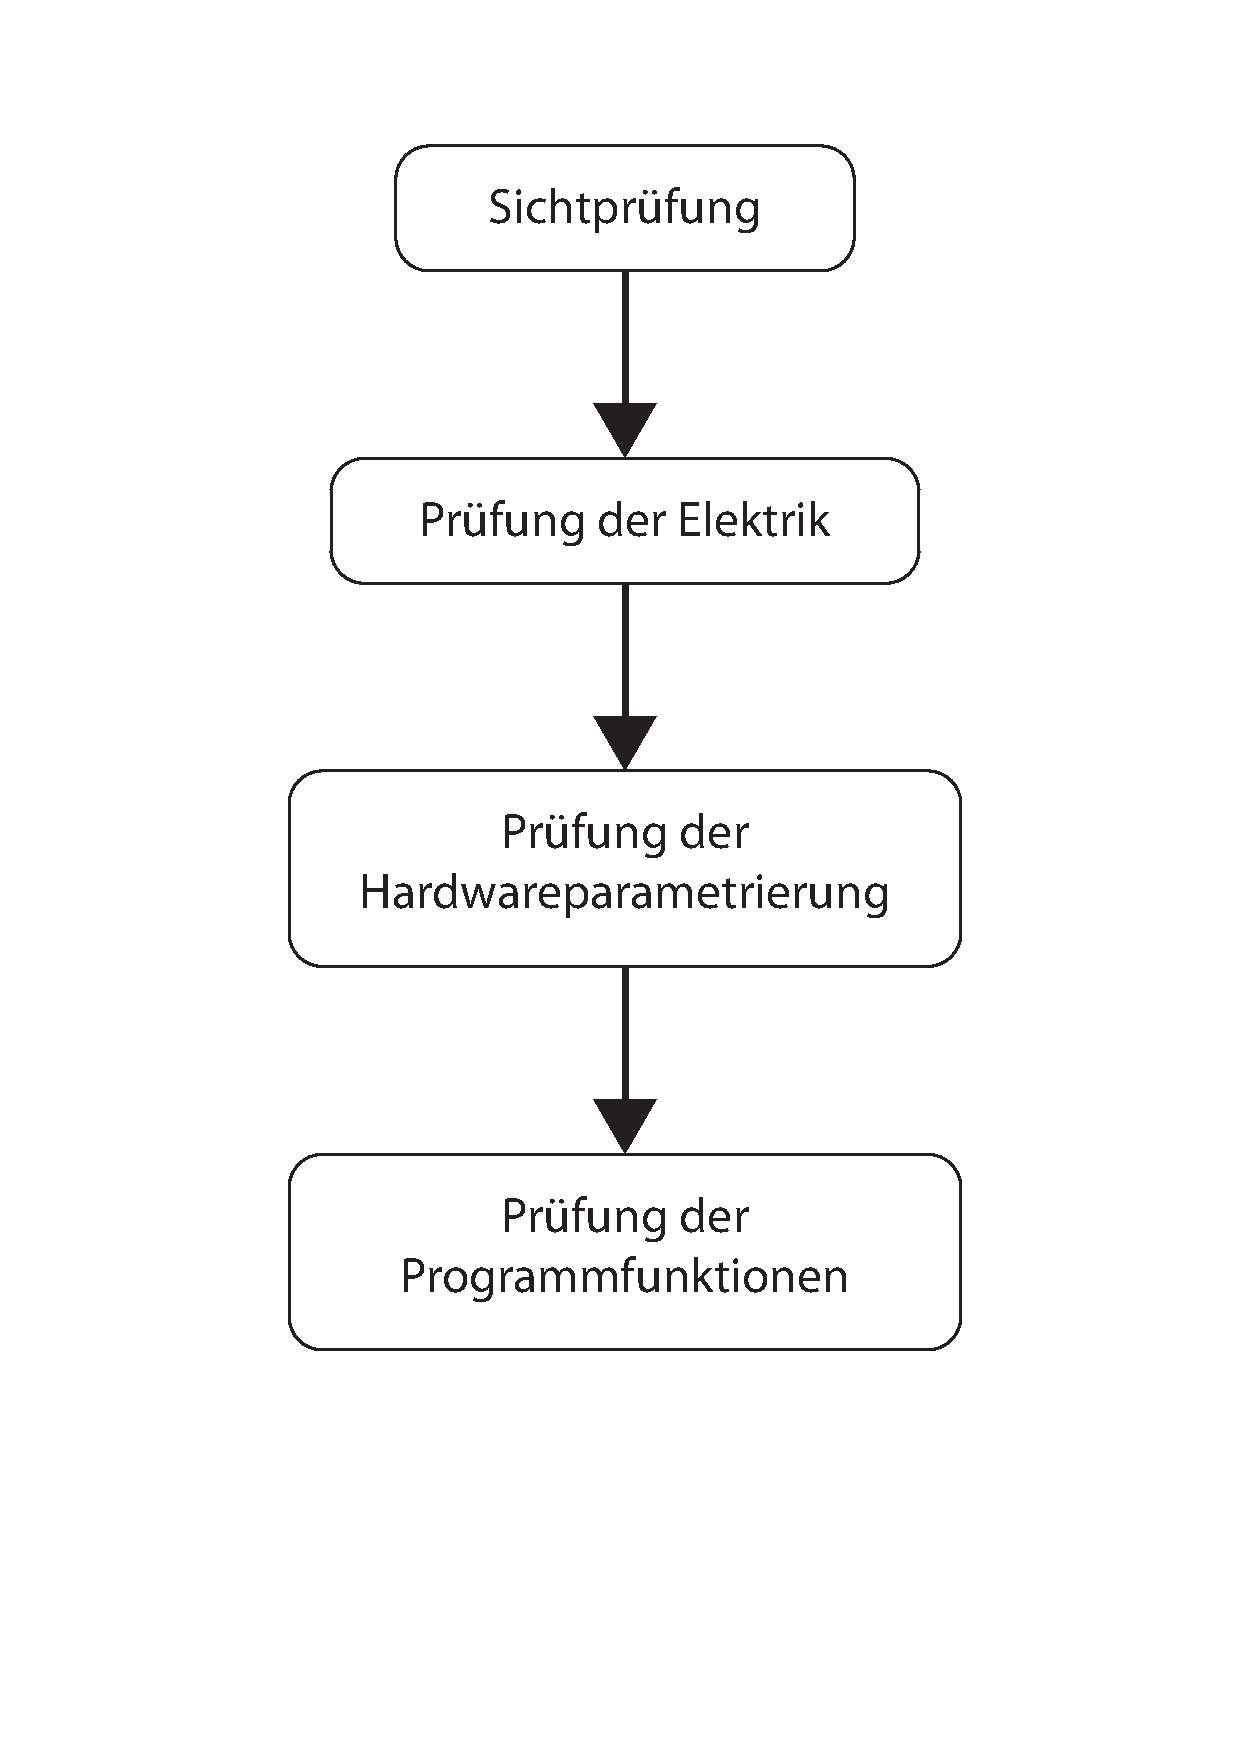
\includegraphics[width=0.5\textwidth]{Images/pruefablauf.pdf}
    \caption[Prüfablauf]{Ablauf zur schrittweisen Verifizierung der Testspezifikationen}
    \label{fig:my-img50}
\end{figure}

Die Protokollierung der Tests erfolgt nach der vorgenommenen Einteilung des dargestellten Diagrammes. Die Einzelnen Punkte werden in den nachfolgenden Unterabschnitten abgearbeitet. Erneut kommt eine tabellarische darstellung zum einsatz, in der einzelne Testfälle mit den Schlüsselwörtern \textbf{bestanden}, \textbf{nicht bestanden} und \textbf{nicht getestet} protokolliert werden. Nicht durchgeführte Tests müssen nachgeholt werden. Ist ein Testfall nicht bestanden, so wird im anschließenden Unterkapitel die Korrektur der Implementierung diskutiert.

\subsubsection{Sichtprüfung}
Vorhandensein Endlagen, Not-Halt-Taster, Lichtvorhang, Bedienelemente, Signalsäule

\subsubsection{Elektrische Prüfung}
Können die Betriebsmittel eingeschalten werden, ist alles richtig verdrahtet?

\subsubsection{Prüfung der Geräteparametrierung}
läuft der sercos, können daten zwischen den PLCs versendet werden, ist der Servoregler eingerichtet, ist das Netzteil eingerichtet, funktionieren die sicheren Ein-/Ausgänge, könne Daten per OPC ausgelesen werden?

\subsubsection{Prüfung der Programmfunktionen}
Führt die Programmierung des Systems zum geplanten Verhalten? 

\end{document}